\documentclass[10pt,a4paper]{amsart}
\usepackage{amsmath,amssymb,amsthm,graphicx}
\usepackage{graphicx}
\usepackage{amssymb}
\usepackage{amsmath}
\newtheorem{theorem}{Theorem}
\newtheorem{question}{Question}
\newtheorem{lemma}[theorem]{Lemma}
\newtheorem{prop}[theorem]{Proposition}
\newtheorem{cor}[theorem]{Corollary}
\newtheorem{conj}[theorem]{Conjecture}
\newtheorem{claim}[theorem]{Claim}
\newtheorem{example}[theorem]{Example}

\theoremstyle{definition}
\newtheorem{definition}[theorem]{Definition}
\newtheorem{remark}[theorem]{Remark}
\newcommand{\und}{\underline}
\newcommand{\ovl}{\overline}
\newcommand{\oi}{\overset{i}}
\newcommand{\zz}{(\mathbb{Z}\slash2\mathbb{Z}) *(\mathbb{Z}\slash2\mathbb{Z})}
\newcommand{\e}{\mathrm{Ends}}
\newcommand{\Z}{\mathbb{Z}}
\newcommand{\F}{\mathbb{F}}
\newcommand{\A}{\mathcal{A}}
\newcommand{\C}{\mathcal{C}}
\newcommand{\V}{\mathcal{V}}
\newcommand{\HF}{\textnormal{HF}}
\DeclareMathOperator{\supp}{supp}
\def\acts{\curvearrowright}

\newcommand{\asi}{\textnormal{asi}}
\newcommand{\dom}{\textnormal{dom}}
\newcommand{\res}{\upharpoonright}
\newcommand{\inv}{^{-1}}
\usepackage{cleveref}
\crefname{originalproposition}{original proposition}{original propositions}
\Crefname{originalproposition}{Original proposition}{Original propositions}
\makeatletter
\newlabel{prop:hcconstruction}{{10}{source}{}{sourcepointer-1}{}}
\newlabel{prop:hcconstruction@cref}{{[originalproposition][0][]10}{[1][0][]source}{}{}{}}
\makeatother
\title{Greedy label sets characterize computable solutions to local problems on forests}
\author{Felix Weilacher}
\date{arxiv:2208.06689v2; CC BY 4.0}
\begin{document}
\maketitle
\noindent\textit{Editorial note.} The counted theorem is the characterization for forests. The author introduces the contrapositive with a stronger tree statement at311-313, but the actual proof explicitly constructs a forest and proves exactly that in Claim356-364. Only the forest conclusion needed by the counted theorem is used; the stronger connectedness assertion is not counted or silently repaired.\par\medskip
\noindent\textit{Editorial note.} The effective-enumeration and least-unused-label conventions referred to as before in315-316 are stated explicitly among the standard prerequisites. The preceding non-full long-path argument is not a premise for this task.\par\medskip
\noindent\textit{Editorial note.} For the finite-reserve choices N0 at322/354 one can make the author free choice of a sufficiently large integer divisible by (2*Delta*|Sigma|)\textasciicircum{}|Sigma|, when |Sigma|>0, so all divisions in active stages are integral. If Sigma is empty, a valid local coloring never occurs and no active-stage division is executed.\par\medskip
\noindent\textit{Editorial note.} All original mathematical proof lines and the two original diagrams are retained. The continuous-coloring proposition301-307, which is outside this claim, is not used.\par\medskip
\noindent\textit{Editorial scope.} One computable-forest characterization theorem, both directions. The nongreedy forest construction and every reserve/decidability argument form the solution. Standard computability enumeration is allowed. The previously published non-full/higher-computability theorem and the unproved stronger connected-tree wording are not additional claims.\par\medskip
\noindent\textit{Allowed standard prerequisites (editorial).}\begin{itemize}
\item Effective enumeration and dovetailing. Use disjoint infinite computable vertex/edge sets X,E in HF, a computable order of HF of type omega, an effective list phi\_t of partial recursive maps X times E to the finite label set, and a computable stage schedule listing each t infinitely often.. The same-source preceding construction185-193 sets these standard conventions.. Enumerate every candidate computable coloring and allocate least unused labels. The nonstandard adversarial forest, reserve invariant and bad local patterns remain solution obligations.
\end{itemize}\medskip
\ifdefined\hypertarget\hypertarget{sourcepointer-1}{}\fi
\noindent\textit{Source reference.} Original proposition 10: sources/weilacher-local-trees-2208.06689v2/source0.tex, source lines 173--175. The references316/354/363/371 point to the earlier construction only for standard effective enumeration, least-unused labels and the same finite-versus-infinite active-stage pattern. These enumeration conventions are explicit standard\_prerequisites; the current proof318-354 provides the entire bad-star/reserve construction,356-364 proves acyclicity and decidable incidence, and370-371 gives the total-coloring contradiction. No non-full path-construction assertion or fullness theorem is needed.\par\medskip
In this paper, we consider locally checkable labeling problems (LCLs) on regular trees. We will use the following formulation of such LCLs from \cite{G+_trees}. Colorings in this formulation are on so-called ``half edges'', and we will need a nonstandard formalization of the notion of a graph to fully accommodate these. Fix $\Delta \geq 2$.

\begin{definition}\label{def:graph}
    A \textit{$\Delta$-regular graph} $G$ with vertex set $X$ and edge set $E$ is a subset $G \subset X \times E$ such that for each $x \in X$, there are exactly $\Delta$ $e \in E$ with $(x,e) \in G$, for each $e \in E$, the number of $x \in X$ with $(x,e) \in G$ is either 1 or 2, and for each $x \neq y$ in $X$, there is at most 1 $e \in E$ with $(x,e),(y,e) \in G$.
    
    An element $(x,e)$ $G$ is called a \textit{half edge incident to} $x$, $x$ an \textit{endpoint} of $e$, and $e$ \textit{incident} to $x$. If a given edge $e$ has two endpoints, say $x,y \in X$, we call it a \textit{true} edge, and say $x$ and $y$ are \textit{adjacent} and that $y$ is a \textit{neighbor} of $x$. In this case we may also identify the half edge $(x,e)$ with the ordered pair $(x,y)$. We will also call the half edges $(x,e)$ and $(y,e)$ the half edges \textit{comprising} $e$. Otherwise we call $e$ a \textit{virtual} edge and $(x,e)$ a \textit{virtual half edge}.
    
    If $x$ is a vertex of $G$, the \textit{degree} of $x$, denoted $\deg(x)$, is the number of neighbors of $x$. Call $G$ \textit{truly} $\Delta$-regular if the degree of each vertex is $\Delta$. This is equivalent to $G$ having no virtual edges.
\end{definition}

We use the definition of adjacency for vertices above to port standard graph theoretic terminology into this model. E.g. path, path distance, cycle, connected component. We call a graph $G$ \textit{acyclic} or a \textit{forest} if it has no cycles. We call a set of vertices $G$-\text{invariant} if it is a union of $G$-connected components. We use $B(-,r)$ to denote the radius $r$ (w.r.t. path distance) neighborhood of a vertex or set of vertices.

Observe also that if our $G$ is truly $\Delta$-regular, the adjacency relation gives a $\Delta$-regular graph on $X$ in the traditional sense, call it $\overline{G}$. In this case the identification in paragraph 2 of the above definition actually gives a bijection between $G$ and $\overline{G}$ where half edges in $G$ go to ordered edges in $\overline{G}$. We can thus identify $G$ and $\overline{G}$ in this case.

We can now describe our LCLs:

\begin{definition}\label{def:lcl}
	An \textit{LCL on $\Delta$-regular graphs} $\Pi$ is a triple $(\Sigma,\mathcal{V},\mathcal{E})$, where $\Sigma$ is a finite set, and $\mathcal{V}$ and $\mathcal{E}$ are sets of size $\Delta$ and $2$, respectively, multisets of labels from $\Sigma$. 
	
	Let $G$ be a $\Delta$-regular graph and $c:G \rightarrow \Sigma$. (That is, $c$ is a labeling of the half edges of $G$.)
	    \begin{itemize}
	        \item If $e$ is a true edge of $G$, write $c(e)$ to denote the size 2 multiset $\{c(x,e),c(y,e)\}$, where $x$ and $y$ are the endpoints of $e$.
	        \item If $x$ is a vertex of $G$, write $c(x)$ to denote the size $\Delta$ multiset of colors given to the half edges meeting $x$.
	    \end{itemize}
    We say $c$ is a \textit{$\Pi$-coloring} of $G$ if for each true edge $e$ of $G$, $c(e) \in \mathcal{E}$, and for each vertex $x$ of $G$, $c(x) \in \mathcal{V}$.
\end{definition}

We now formally describe some of the settings which were described informally above. In (3) below and throughout the paper, $\HF$ denotes the set of hereditarily finite sets, which we use as our domain for discussing computability. Note that the definitions below make sense for general classes of graphs, but in this paper we are chiefly concerned with complexity classes for acyclic graphs.

\begin{definition}
	Let $\Pi = (\Sigma,\mathcal{V},\mathcal{E})$ be an LCL on $\Delta$-regular graphs.
	\begin{enumerate}
		\item We call a truly $\Delta$-regular graph $G$ \textit{Borel} if its vertex set $X$ is a Polish space and the associated $\overline{G}$ (see the comment after Definition \ref{def:graph}) is Borel in $X \times X$. We call a coloring $c:G \rightarrow \Sigma$ \textit{Borel} if it is Borel as function on $\overline{G} \subset X \times X$. We say $\Pi$ is in the class BAIRE if every acyclic such $G$ admits a Borel $\Pi$-coloring off a $G$-invariant meager Borel subset of vertices. I.e, there is a $G$-invariant comeager Borel set $C \subset X$ such that the graph identified with $\overline{G} \cap (C \times C)$ admits a Borel $\Pi$-coloring.
		
		\item (\cite{bernshteyn_continuous},\cite{BCG_Trees2}) We call a Borel $\Delta$-regular graph $G$ as in (1) \textit{continuous} if $X$ is zero-dimensional and for any clopen $U \subset X$, the set of neighbors of elements of $U$ is clopen. We call a coloring $c: G \rightarrow \Sigma$ \textit{continuous} if it continuous as a function on $\overline{G} \subset X \times X$ with the subspace topology. We say $\Pi$ is in the class CONTINUOUS if every acyclic such $G$ admits a continuous $\Pi$-coloring.
		
		
		\item We call a $\Delta$-regular graph $G$ \textit{computable} if its vertex and edge sets $X$ and $E$ are computable subsets of $\HF$ and $G$ is a computable subset of $X \times E$. We call a coloring $c : G \rightarrow \Sigma$ computable if it is computable as a function (we may of course assume $\Sigma \subset \HF$.) We say $\Pi$ is in the class COMPUTABLE if every computable acyclic $\Delta$-regular graph admits a computable $\Pi$-coloring.
	
	
        \item We call a computable $\Delta$-regular graph $G$ as in (3) \textit{highly computable} if the degree function $\deg:X \rightarrow \omega$ is computable. Since there are $\Delta$ edges incident to each $x \in X$ and $\deg(x)$ is the number of true such edges, this is equivalent to the set of true edges being computable. In particular, truly $\Delta$-regular computable graphs are highly computable. We say $\Pi$ in in the class HCOMP if every highly computable acyclic $\Delta$-regular graph admits a computable $\Pi$-coloring.
    \end{enumerate}
\end{definition}

\begin{definition}\label{def:greedy}
    Let $\Pi = (\Sigma,\mathcal{V},\mathcal{E})$ be an LCL on $\Delta$-regular graphs. Let $\Sigma' \subset \Sigma$. We say $\Sigma'$ is \textit{greedy} if the following holds: Let $k \in \{0,\ldots,\Delta\}$, and consider the $\Delta$-regular tree $H$ with vertices $x$ and $y_i$ for $i < k$ with $x$ and $y_i$ adjacent for each $i$ and all other edges being virtual. Precolor each half edge $(y_i,x)$ with a label from $\Sigma'$. Then this can be extended to a $\Pi$-coloring of $H$ such that $c(x,e) \in \Sigma'$ for each virtual edge $e$ incident to $x$. (See Figure \ref{fig:greedy}.) We say $\Pi$ is \textit{greedy} if it admits some greedy $\Sigma'$.
\end{definition}

\begin{figure}
    \centering
    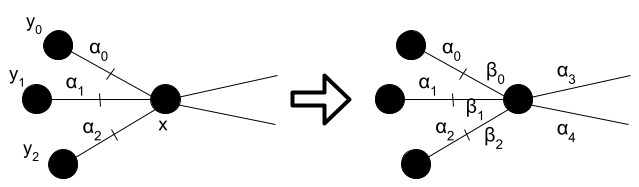
\includegraphics[width = 0.9\textwidth]{Greedy.png}
    \caption{An illustration of Definition \ref{def:greedy} with $\Delta = 5$ and $k = 3$. True edges are divided with slashes to show the two half edges comprising them. The left hand figure is given, and the right hand figure is the needed extension. The $\alpha$'s are colors from $\Sigma'$, whereas the $\beta$'s can be any elements of $\Sigma$. Definition \ref{def:greedy} also technically asks for colors for the other half edges incident to the $y_i$'s, but these do not turn out to be relevant and so are not drawn.}
    \label{fig:greedy}
\end{figure}

\begin{theorem}\label{thm:ciffgreedy}
    An LCL on $\Delta$-regular graphs is in COMPUTABLE if and only if it is greedy.
\end{theorem}

\begin{prop}\label{prop:greedytocomp}
        Let $\Pi = (\Sigma,\V,\mathcal{E})$ be an LCL on $\Delta$-regular graphs, and assume $\Pi$ is greedy. Then any computable $\Delta$-regular graph admits a computable $\Pi$-coloring.
\end{prop}

\begin{proof}
    Let $G$ be such a graph, say with vertex and edge sets $X$ and $E$ respectively. WLOG $X \subset \omega$. Let $\Sigma' \subset \Sigma$ be greedy. We will recursively define our coloring $c$ in $\omega$ stages. At stage $n \in \omega$, we will color exactly the half edges incident to $n$ if $n \in X$, and do nothing otherwise. We will maintain that if $e \in E$ is such that exactly one of the half edges comprising $e$ has been colored so far, then it gets a color from $\Sigma'$.
    
    We now describe stage $n$ if $n \in X$: Let $y_i$ for $i < k$ be the neighbors of $n$ less than $n$. Then by inductive hypothesis, $c(y_i,n) \in \Sigma'$ for each $i$, and the $\Delta-k$ other incident edges to $x$, say $e_j$ for $j < \Delta - k$, not having a $y_i$ as their other endpoint have not been touched. Thus, by the definition of greedy, we may color the half edges incident to $x$ so that $c(x,e_j) \in \Sigma'$ for each $j$, thus maintaining our inductive hypothesis. 
\end{proof}

We now turn to the forward direction of \ref{thm:ciffgreedy}. Again we prove the contrapositive:

\begin{proof}
    Our construction will closely follow that in the proof of Proposition \ref{prop:hcconstruction}. Fix $X,E$ and the $\phi_t$'s as before. Once again, we will be recursively constructing a sequence of $\Delta$-regular forests with finite vertex sets, but really building a sequence of $\omega$ forests in parallel as kept track of by a recursively defined function $C:X \rightarrow \omega$. We will use the term ``new'' for added vertices and edges in the same way. Call the forest we are building $T$.
    
    Since $\Pi$ is not greedy, for every $\Sigma' \subset \Sigma$, there is a $k \in \{0,\ldots,\Delta\}$ and a sequence $\alpha_0,\ldots,\alpha_{k-1}$ from $\Sigma'$ witnessing that $\Sigma'$ is not greedy. That is, such that in the situation of Definition \ref{def:greedy}, if this $k$ is used and each half edge $(y_i,x)$ is given the color $\alpha_i$, then if this is extended to a $\Pi$-coloring of $H$, there is some virtual half edge $(x,e)$ such that $c(x,e) \not\in \Sigma'$. Fix choices of such $k$ and $(\alpha_i)_{i < k}$ for each $\Sigma'$ and call them \textit{bad} for $\Sigma'$.
    
    Again, let us fix $t \in \omega$ and describe the $\omega$ steps in the construction of $T \res C\inv(t)$.
    
    The 0-th stage will be similar: Fix a very large $N_0 >> |\Sigma|$ to be determined later, independent of $t$. In the 0-th stage, place $N_0$ new vertices, say $w_0,\ldots,w_{N_0-1}$, in $C\inv(t)$, and give each $\Delta$ new virtual incident edges.
    
    We also initialize several variables: Set $\Sigma' = \emptyset$ and $N = N_0$. Also set $x_i = w_i$ for each $i < N$.
    
    At the start of an arbitrary successor stage, say $m+1$, suppose we have some $\Sigma' \subset \Sigma$,$N \in \omega$ very large, and vertices $x_i$ for $i < N$ and virtual half edges $(y_i^\alpha,e_i^\alpha)$ for $i < N$ and $\alpha \in \Sigma'$ such that:
    \begin{enumerate}
        \item The $x_i$'s and $y_i^\alpha$'s all lie in distinct $C\inv(t)$-components.
        \item For each $i$, if $\phi_t$ restricted to half edges meeting $B(x_i,1)$ gives a $\Pi$-coloring, there must be some virtual edge $e$ incident to $x$ with $\phi_t(x,e) \not\in \Sigma'$.
        \item For each $i$ and $\alpha$, $\phi_t(y_i^\alpha,e_i^\alpha) = \alpha$.
    \end{enumerate}
    
Note that this is all satisfied after stage 0.

We start our successor stage by running the Turing machine computing $\phi_t$ for $m$ steps on all the half edges meeting each $B(x_i,1)$. (Note that we can compute $B(x_i,1)$ since our vertex set so far is finite.)

If $\phi_t$ fails to converge in $\leq m$ steps on one of these inputs, or if it converges on all of them but the result fails to be a $\Pi$-coloring of some $B(x_i,1)$, we do nothing. We call this the ``uninteresting case''.

The ``interesting case'' is of course if $\phi_t$ does converge on all these inputs in $\leq m$ steps, and the result is a $\Pi$-coloring for each $B(x_i,1)$. In this case by condition (2) above, there is a virtual edge $f_i$ for each $i < N$ meeting $x_i$ with $\phi_t(x_i,f_i) \not\in \Sigma'$. Let $\beta \in \Sigma \setminus \Sigma'$ such that $\phi_t(x_i,f_i) = \beta$ for at least $N/|\Sigma|$ $i$'s. Update $\Sigma'$ to $\Sigma' \cup \{\beta\}$.

\begin{figure}
    \centering
    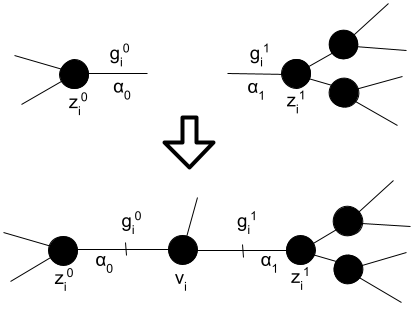
\includegraphics[width = 0.6\textwidth]{Greedy_Joining.png}
    \caption{The ``interesting case'' for a step of the construction for a fixed $t$ with $\Delta = 3$. The top and bottom image represent the before and after states respectively.}
    \label{fig:gj}
\end{figure}

Let $k$ and $\alpha_0,\ldots,\alpha_{k-1} \in \Sigma'$ be bad for $\Sigma'$. Between the $(x_i,f_i)$'s and the $(y_i^\alpha,e_i^\alpha)$'s, and using condition (1) above, we can chose virtual half edges $(z_i^j,g_i^j)$ for $i < M := N / (\Delta |\Sigma|)$ such that the $z_i^j$'s all lie in distinct $C\inv(t)$-components and $\phi_t(z_i^j,g_i^j) = \alpha_j$ for each $j < k$. 

Now for each $i < M/2$, Let $v_i$ be a new vertex and add it as an endpoint to $g_i^j$ for each $j$, making all these edges true. Then, to maintain $\Delta$-regularity, add $\Delta-k$ new virtual incident edges to $v_i$. This is shown in Figure \ref{fig:gj}. 

We can now finish this stage of the construction with the updated value of $N$ being $M/2$. First set $x_i = v_i$ for each $i$. Condition(2) is then satisfied by definition of bad. We now define the $(y_i^\alpha,e_i^\alpha)$'s. If $\alpha = \alpha_j$ for some $j$, we can use the unused $(z_i^j,g_i^j)$'s. Else, if $\alpha = \beta$ we can use the first $M/2$ $(x_i,f_i)$'s, and if not, the first $M/2$ $(y_i^\alpha,e_i^\alpha)$'s from the previous stage of the construction.

Thus the description of the construction is complete. As in the proof of Proposition \ref{prop:hcconstruction}, it will be significant that the interesting case cannot occur more than $|\Sigma|$ times for a fixed $t$ (since $|\Sigma'|$ increases by one each time it does). As in that proof, the first application of this is that it tells us what to pick for $N_0$: We can take $N_0 > (2\Delta |\Sigma|)^{|\Sigma|}$, since $2\Delta|\Sigma|$ is by how much the value of $N$ was divided each time the interesting case occurred. 

\begin{claim}\label{claim:Tcomp2}
$T$ is a computable $\Delta$-regular forest.
\end{claim}

\begin{proof}
    At each stage in the construction, we either added new trees as components, did nothing, or joined separate components at a single new vertex. Thus $T$ is acyclic.
    
    $T$ has vertex and edge set $X$ and $E$ for the same reason as in the proof of Proposition \ref{prop:hcconstruction}. Also, since we maintain $\Delta$-regularity at each stage in the construction, to check if a pair $(x,e) \in X \times E$ is in $T$, we can run the construction until $x$ is added as a vertex, and then check if $e$ is one of its incident edges. Thus $T$ is computable.
\end{proof}

\begin{claim}
$T$ admits no computable $\Pi$-coloring.
\end{claim}

\begin{proof}
    Exactly as in the proof of Proposition \ref{prop:hcconstruction}, if some $\phi_t$ were a $\Pi$-coloring of $T$, we could conclude that the interesting case occurs infinitely often for this $t$, contradicting the statement before Claim \ref{claim:Tcomp2}.
\end{proof}

\end{proof}

\bibliographystyle{plain}
\bibliography{main}
\end{document}
